\newpage

\section*{Kinematics:}

\begin{center}
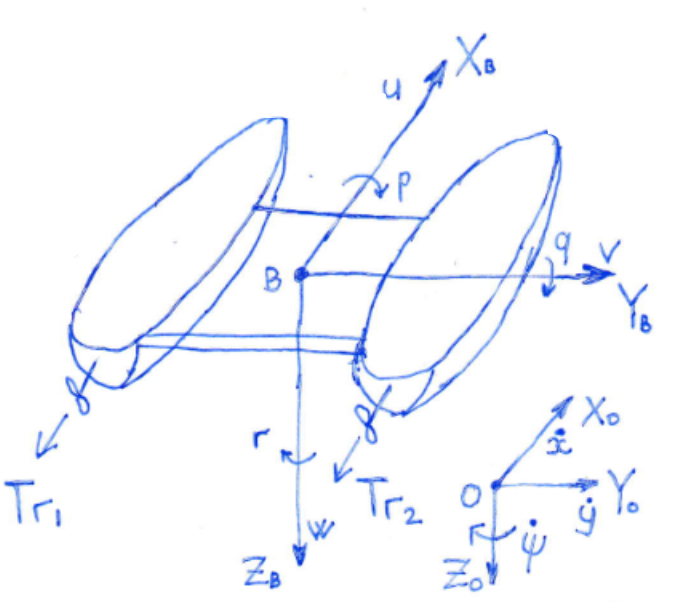
\includegraphics[width=0.6\textwidth]{img/lodka-clear.png}\\
\end{center}

3-DOF: \\

u(surve); \\

v(sway); \\

w(heave) = 0; \\

p(roll) = 0; \\

q(pitch) = 0; \\

r(yaw)
\begin{center}
  %\normalise
\begin{equation*}
Body: \nu = \begin{bmatrix}
u \\
v \\
r
\end{bmatrix};\quad Earth-fixed: \eta = \begin{bmatrix}
 x \\
 y \\
 \psi
 \end{bmatrix}
\end{equation*}
\end{center}
\begin{equation*}
\Dot{\eta} = J(\eta)\nu, \quad J = \begin{bmatrix}
cos\psi & -sin\psi & 0 \\
sin\psi & cos\psi & 0 \\
0 & 0 & 1
 \end{bmatrix}
\end{equation*}

%\noindent{\rule{4cm}{0.4pt}}

\newpage
\section*{Уравнения Кирхгофа:}
\large
\begin{equation*}
 \begin{cases}
   \frac{d}{dt}(\frac{\partial T}{\partial \nu_1}) + S(\nu_2)\frac{\partial T}{\partial \nu_1} = \tau_1\\
   \frac{d}{dt}(\frac{\partial T}{\partial \nu_2}) + S(\nu_2)\frac{\partial T}{\partial \nu_2} + S(\nu_1)\frac{\partial T}{\partial \nu_1} = \tau_2
 \end{cases}
 \end{equation*}

\begin{equation*}
T = \frac{1}{2}\nu^TM\nu - \text{кинетическая энергия};\; M - \text{mass matrix};\; S(*) - \text{skew-symmetric matrix}
\end{equation*}

\begin{equation*}
\nu_1 = \begin{bmatrix}
u & v & w
 \end{bmatrix}^T;\; \nu_2 = \begin{bmatrix}
 p & q & r
  \end{bmatrix}^T;\; \tau_1 = \begin{bmatrix}
X & Y & Z
 \end{bmatrix} - \text{силы};\; \nu_2 = \begin{bmatrix}
 K & M & N
  \end{bmatrix}^T - \text{моменты}; \\
\end{equation*}

\noindent{\rule{4cm}{0.4pt}} \\

Без учета added mass:
\begin{equation*}
M = \begin{bmatrix}
m & 0 & 0 \\
0 & m & 0 \\
0 & 0 & I_{zz}
\end{bmatrix}; \quad T = \frac{1}{2}(mu^2 + mv^2 + I_{zz}t^2);\;
\end{equation*}

\begin{equation*}
I_{zz} = I_{zcuboid} + 2(I_{xelipsoid} + m_{elipsoid}\;d_{axis}^2) - \text{аппроксимация коробкой и эллипсами}
\end{equation*}

\begin{equation*}
S(\nu_1) = \begin{bmatrix}
0 & 0 & v \\
0 & 0 & -u \\
-v & u & 0
\end{bmatrix};\; S(\nu_2) = \begin{bmatrix}
0 & -r & 0 \\
r & 0 & 0 \\
0 & 0 & 0
\end{bmatrix}
\end{equation*}

\noindent{\rule{4cm}{0.4pt}}

\begin{equation*}
\begin{bmatrix}
m\Dot{u} - mvr \\
m\Dot{v} + mur \\
I_{zz}\Dot{r}
\end{bmatrix} = \begin{bmatrix}
X \\
Y \\
N
\end{bmatrix} => M\Dot{\nu} + C(\nu)\nu = \tau
\end{equation*}

\begin{equation*}
C(\nu) = \begin{bmatrix}
0 & 0 & -mv \\
0 & 0 & mu \\
mv & -mu & 0
\end{bmatrix};\; \tau = \begin{bmatrix}
X \\
Y \\
N
\end{bmatrix}
\end{equation*}

